\documentclass{estilo}
\usepackage[spanish]{babel}
\usepackage{graphicx}
\usepackage{float}
\usepackage{amsmath}        % para los vectores columnas
\usepackage{amsfonts}       % para las negrita de pizarra
\usepackage{amssymb}        % para simbolos matematicos
\usepackage{hyperref}       % para utilizar referencias
\usepackage{multirow}       % para las tablas
\usepackage{dsfont}
\usepackage{listings}
\usepackage{xcolor}
\definecolor{codegreen}{rgb}{0,0.6,0}
\definecolor{codegray}{rgb}{0.5,0.5,0.5}
\definecolor{codepurple}{rgb}{0.58,0,0.82}
\definecolor{backcolour}{rgb}{0.95,0.95,0.92}
\lstdefinestyle{mystyle}{
    backgroundcolor=\color{backcolour},
    commentstyle=\color{codegreen},
    keywordstyle=\color{magenta},
    numberstyle=\tiny\color{codegray},
    stringstyle=\color{codepurple},
    basicstyle=\ttfamily\footnotesize,
    breakatwhitespace=false,
    breaklines=true,
    captionpos=b,
    keepspaces=true,
    numbers=left,
    numbersep=5pt,
    showspaces=false,
    showstringspaces=false,
    showtabs=false,
    tabsize=2
}
\lstset{style=mystyle}

\usepackage{enumitem,multicol,setspace}
\newcounter{subenum}[enumi] % para las multicolumnas
\renewcommand{\thesubenum}{\arabic{subenum}}
\usepackage[nomessages]{fp}
\FPeval\thecolwidth{round(1/4:4)}% Specify number of columns -> column width
\newcommand{\newitem}[1]{%
  \refstepcounter{subenum}%
  \parbox{\dimexpr\thecolwidth\linewidth-.5\columnsep}{%
    \makebox[\labelwidth][r]{(\thesubenum)\hspace*{\labelsep}}%
    #1}\hfill%
}

\usepackage{scalerel,stackengine} % para el sombrero
\stackMath
\newcommand\rhat[1]{%
\savestack{\tmpbox}{\stretchto{%
  \scaleto{%
    \scalerel*[\widthof{\ensuremath{#1}}]{\kern-.6pt\bigwedge\kern-.6pt}%
    {\rule[-\textheight/2]{1ex}{\textheight}}%WIDTH-LIMITED BIG WEDGE
  }{\textheight}% 
}{0.5ex}}%
\stackon[1pt]{#1}{\tmpbox}%
}
\parskip 1ex

\usepackage{mathtools}      % floor y ceil
\DeclarePairedDelimiter\ceil{\lceil}{\rceil}
\DeclarePairedDelimiter\floor{\lfloor}{\rfloor} 

\usepackage[style=authoryear-comp]{biblatex}


\begin{document}
\maketitle

\justifying{}

\newpage
\section{Introducci\'on}

En el presente trabajo pr\'actico se realiza un analisis de un algoritmo por
\textit{Programaci\'on Din\'amica} para resolver un problema de maximizaci\'on.

\section{Consideraciones}

Un cronograma de entrenamiento indica cuanto esfuerzo demanda el entrenamiento
de cada d\'ia. Se puede calcular la ganancia de cada d\'ia como el m\'inimo
entre el esfuerzo requerido por el entrenamiento para ese d\'ia $\left( e_i
\right)$, y la eneg\'ia que tienen los jugadores en ese d\'ia $\left( j
\right)$ o $0$ si descansan.

La energ\'ia que tienen los jugadores en un d\'ia determinado depende de hace
cuantos d\'ias descansaron por \'ultima vez y est\'a dada por la secuencia
$\mathcal{S}$:

\begin{equation*}
    \mathcal{S} = s_1, s_2, ..., s_n
\end{equation*}
\begin{equation*}
    \text{con } s_1 \ge s_2 \ge ... \ge s_n
\end{equation*}

\section{Problema}

Dada la secuencia de energ\'ia disponible desde el \'ultimo descanso
$\mathcal{S}$, y el esfuerzo/ganancia de cada d\'ia, determinar la m\'axima
cantidad de ganancia que se puede obtener de los entrenamientos, considerando
posibles descansos.

\subsection{Ecuaci\'on de Recurrencia}

Los jugadores comienzan descansados y sin ninguna ganancia:

\begin{equation*}
    \mathcal{G} \left( 0, 0 \right) = 0
\end{equation*}

Si eligen descansar en el d\'ia $k$, al d\'ia siguiente se renueva su
energ\'ia, por lo que lo mejor ser\'a maximizar la ganancia del d\'ia anterior:

\begin{equation*}
    \mathcal{G} \left( 0, k \right) = \max_{0 \le i < k} \left( \mathcal{G} \left( i, k - 1 \right) \right)
\end{equation*}

Por otro lado, si no descansan la ganancia para ese d\'ia depende de su
energ\'ia y de la ganancia del d\'ia anterior:

\begin{equation*}
    \mathcal{G} \left( i, k \right) = \mathcal{G} \left( i - 1, k - 1 \right) + \min \left( s_i, e_k \right)
\end{equation*}

Lo que nos deja con la siguiente ecuaci\'on de recurrencia:

\begin{equation}
    \begin{cases}
        \mathcal{G} \left( 0, 0 \right) = 0\\
        \mathcal{G} \left( 0, k \right) = \max_{0 \le i < k} \left( \mathcal{G} \left( i, k - 1 \right) \right)\\
        \mathcal{G} \left( i, k \right) = \mathcal{G} \left( i - 1, k - 1 \right) + \min \left( s_i, e_k \right)\\
    \end{cases}
\end{equation}

donde $\mathcal{G} \left( 0, n + 1 \right)$ es la soluci\'on al problema.

\newpage
\justifying{
\hypertarget{res}{\section*{Resolución}}
\subsection{Algoritmo}

Para encontrar $\mathcal{G} \left( 0, n + 1 \right)$, proponemos el siguiente
algoritmo por \textit{Programaci\'on Din\'amica}:

Para cada d\'ia, considerar la posibilidad de haber descansado por \'ultima
vez en cualquiera de los d\'ias anteriores, y calcular la ganancia
correspondiente. Adem\'as, considerar que se puede descansar en el mismo d\'ia,
en cuyo caso la ganancia m\'axima del d\'ia anterior es la ganancia para ese
d\'ia.

De esta forma podemos calcular las posibles ganancias de cada d\'ia de
entrenamiento utilizando \'unicamente las posibles ganancias del d\'ia
anterior. Como pudieron haber descansado por \'ultima vez en cualquiera de los
d\'ias anteriores, los cuales son a lo sumo $n$, la complejidad espacial de
nuestro algoritmo es $\mathcal{O}(n)$.

\subsection{Implementaci\'on}
\label{sec:implementacion}

\lstinputlisting[language=Python]{code/solution.py}

La ecuaci\'on de recurrencia que corresponde a este algoritmo es:
\begin{equation*}
    \mathcal{T}(n) = \mathcal{T}\left(n - 1\right) + \mathcal{O}\left(n\right)
\end{equation*}

Esto es porque en cada iteraci\'on calculamos el m\'aximo de un arreglo de
tama\~no $n$ $\left( \mathcal{O}(n) \right)$, e iteramos por el mismo
realizando operaciones de tiempo constante $\left( \mathcal{O}(n) \right)$.

Aplicando en teorema maestro, o multiplicando por la cantidad de
entrenamientos, nos queda que la complejidad es $\mathcal{O}(n^2)$.
 
\subsection{Reconstrucci\'on}

Para encontrar el camino que maximiza el esfuerzo alcanza con tener el estado final
del arreglo de ganancias propuesto \hyperref[sec:implementacion]{anteriormente},
ya que con este se pueden reconstruir todos los estados anteriores del mismo.
Considerando un arreglo de ganancias para el día $n$ con un máximo en la
posici\'on $k$ se da que:
\begin{equation*}
    ganancias[k] = \mathcal{G} ( 0, k + 1 ) + \sum_{i=1}^{n-k} \min (s_i, e_{k+i})
\end{equation*}
    Que es equivalente a decir que el camino cumple con haber descanzado el día
$k$ y trabajado todos los días posteriores.\\

    Con esto en mente, alcanza con restarle la sumatoria 
$\sum_{i=1}^{n-k} \min (s_i, e_{k+i})$ al elemento en la posici\'on $k$ para
recuperar el valor que ten\'ia en el d\'ia $k$.\\
Generalizando: el valor en el \'indice $j$ para el d\'ia $k$, con $j \leq k$,
puede recuperarse con:
\begin{equation*}
    ganancias[j] - \sum_{i=1}^{n-k} \min (s_{k+i-j}, e_{k+i})
\end{equation*}

    Una vez reconstruido el arreglo para el d\'ia $k$, y considerando la
equaci\'on para $\mathcal{G} ( 0, k )$ \eqref{eq:g_{0k}}, tenemos que el problema
se reduce a una versi\'on m\'as peque\~na de s\'i mismo. 

\newpage
\section{Mediciones}

Se realizaron mediciones en base a crear arreglos de diferentes largos con
valores de energ\'ia consumida por entrenamiento y energ\'ias disponibles en el
rango de $[1,100]$ (como en los casos de prueba provistos por la catedra),
yendo de 10 en 10 elementos, donde los elementos en cada caso fueron generados
por los valores pseudoaleatorios del lenguaje (el m\'odulo \texttt{random}).

\begin{figure}[H]
    \centering % comparar el tiempo de ejecucion con (n^2)
    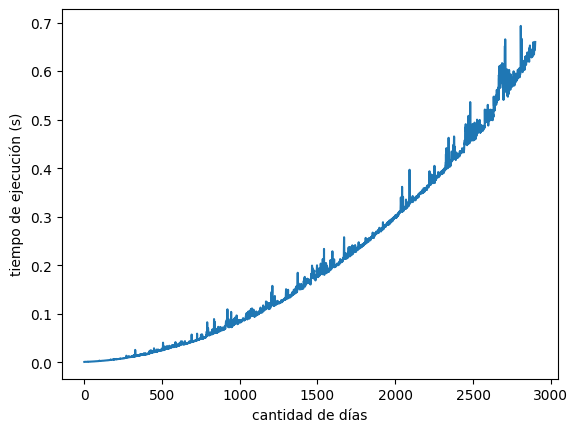
\includegraphics[width=1\textwidth]{img/tiempos.png}
\end{figure}

Como se puede apreciar, el algoritmo tiende a $\mathcal{O}\left( n^2 \right)$.

\section{Conclusiones}

La soluci\'on propuesta plantea la utilización del día anterior para el calculo de un entrenamiento óptimo. 
Como solo prescindimos del entrenamiento del d\'ia anterior para calcular nuestro d\'ia actual, la \textit{memoization} requerida es de espacio lineal.

Al haber planteado un algoritmo de complejidad exponencial cuadratica, no podemos decir que la soluci\'on es veloz, pero sin embargo es la m\'as \'optima posible, el m\'etodo de reconstrucci\'on por su parte s\'i es r\'apido, ya que tiene complejidad lineal.

Destacamos que nuestro algorimo no considera la condicion inicial de $e_i >= e_{i+1}$, por lo que nuestro programa podria hayar soluciones para casos en los que no este dada esta restricci\'on.

}


\newpage
\end{document}
